%% Creator: Inkscape inkscape 0.92.2, www.inkscape.org
%% PDF/EPS/PS + LaTeX output extension by Johan Engelen, 2010
%% Accompanies image file 'saut1.eps' (pdf, eps, ps)
%%
%% To include the image in your LaTeX document, write
%%   \input{<filename>.pdf_tex}
%%  instead of
%%   \includegraphics{<filename>.pdf}
%% To scale the image, write
%%   \def\svgwidth{<desired width>}
%%   \input{<filename>.pdf_tex}
%%  instead of
%%   \includegraphics[width=<desired width>]{<filename>.pdf}
%%
%% Images with a different path to the parent latex file can
%% be accessed with the `import' package (which may need to be
%% installed) using
%%   \usepackage{import}
%% in the preamble, and then including the image with
%%   \import{<path to file>}{<filename>.pdf_tex}
%% Alternatively, one can specify
%%   \graphicspath{{<path to file>/}}
%% 
%% For more information, please see info/svg-inkscape on CTAN:
%%   http://tug.ctan.org/tex-archive/info/svg-inkscape
%%
\begingroup%
  \makeatletter%
  \providecommand\color[2][]{%
    \errmessage{(Inkscape) Color is used for the text in Inkscape, but the package 'color.sty' is not loaded}%
    \renewcommand\color[2][]{}%
  }%
  \providecommand\transparent[1]{%
    \errmessage{(Inkscape) Transparency is used (non-zero) for the text in Inkscape, but the package 'transparent.sty' is not loaded}%
    \renewcommand\transparent[1]{}%
  }%
  \providecommand\rotatebox[2]{#2}%
  \ifx\svgwidth\undefined%
    \setlength{\unitlength}{458.93788937bp}%
    \ifx\svgscale\undefined%
      \relax%
    \else%
      \setlength{\unitlength}{\unitlength * \real{\svgscale}}%
    \fi%
  \else%
    \setlength{\unitlength}{\svgwidth}%
  \fi%
  \global\let\svgwidth\undefined%
  \global\let\svgscale\undefined%
  \makeatother%
  \begin{picture}(1,0.55996795)%
    \put(0,0){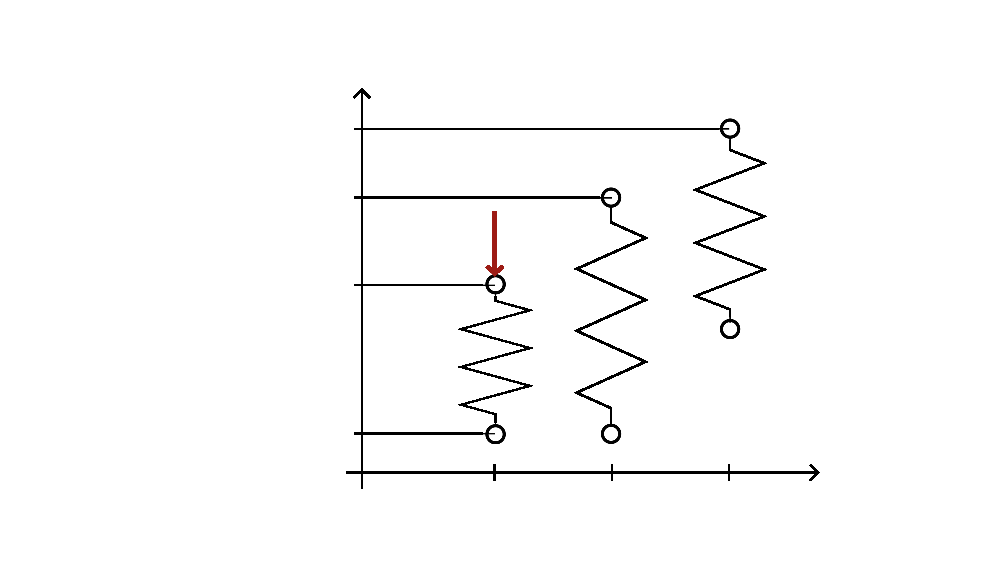
\includegraphics[width=\unitlength]{images_2ddl/saut1.eps}}%
    \put(0.35332121,0.50424636){\color[rgb]{0,0,0}\makebox(0,0)[lb]{\smash{$y$}}}%
    \put(0.85079889,0.07843695){\color[rgb]{0,0,0}\makebox(0,0)[lb]{\smash{$t$}}}%
    \put(0.44868441,0.03798154){\color[rgb]{0,0,0}\makebox(0,0)[lb]{\smash{$t<-t_0$}}}%
    \put(0.59510438,0.04003324){\color[rgb]{0,0,0}\makebox(0,0)[lb]{\smash{$t=0$}}}%
    \put(0.71660123,0.03978188){\color[rgb]{0,0,0}\makebox(0,0)[lb]{\smash{$t=t_f$}}}%
    \put(0.31206609,0.11596114){\color[rgb]{0,0,0}\makebox(0,0)[lb]{\smash{$0$}}}%
    \put(0.12576987,0.27218246){\color[rgb]{0,0,0}\makebox(0,0)[lb]{\smash{$2R-\dfrac{F}{k}-\dfrac{m_r g}{2k}$}}}%
    \put(0.19576987,0.36438468){\color[rgb]{0,0,0}\makebox(0,0)[lb]{\smash{$2R+\dfrac{m_r g}{2k}$}}}%
    \put(0.25429501,0.44056847){\color[rgb]{0,0,0}\makebox(0,0)[lb]{\smash{$y_{1,max}$}}}%
    \put(0.51238222,0.3284082){\color[rgb]{0.61568627,0.10588235,0.07843137}\makebox(0,0)[lb]{\smash{$F$}}}%
  \end{picture}%
\endgroup%
